\documentclass[11pt]{article}
\usepackage{setspace}
\usepackage{graphicx}
\graphicspath{{../diagrams/networks/}{../diagrams/display-trees/}}
\usepackage{subfigure}
\usepackage{lscape}
\usepackage{flafter}  % Don't place floats before their definition
\usepackage{bm}  % Define \bm{} to use bold math fonts
\usepackage{amsmath}
\usepackage{amsfonts}
\usepackage{amssymb}
\usepackage{MnSymbol}
\usepackage{url}
\usepackage{natbib}
\usepackage{pmboxdraw}
\usepackage{float}
\usepackage{fancyvrb}
\usepackage{bera}
\usepackage[section]{placeins}
%\usepackage{fullpage}
\bibliographystyle{cbe}
\citestyle{aa}
%\usepackage{algorithmic}
%\usepackage[vlined,algochapter,ruled]{algorithm2e}
\usepackage[vlined,ruled]{algorithm2e}
\usepackage{listings}% http://ctan.org/pkg/listings
\lstset{
  basicstyle=\ttfamily,
  mathescape
}
\SetKwComment{Comment}{$\triangleright\ $}{}

%ROOT PRIORS?
%Add Giribet and Wheeler arth, ratchet cite, Arango sea spiders

\title{Algorithmic Descriptions and Pseudo-Code for Phylogenetic Component Graphs}
\author{Ward C. Wheeler\\
		%Richard Gilder Graduate School,\\
		Division of Invertebrate Zoology,\\
		American Museum of Natural History,\\
		Central Park West @ 79th Street,\\
		New York, NY 10024-5192,\\
		USA,\\
		wheeler@amnh.org}
	%\date{}
\begin{document}

\maketitle
\begin{abstract}
	Algorithmic Descriptions and Pseudo-Code for network operations on Phylogenetic Component Graphs (PCG).
\end{abstract}
%\newpage
\tableofcontents
%\newpage

%\doublespacing
\section{Introduction} \label{Introduction}
This document contains the descriptions and pseudo-code for core  Phylogenetic Component Graphs (PCG) algorithms.  
This is designed to serve both as documentation for the code and a development tool. 
We have tried to keep the style as consistent as possible, Functional-type statements (\textit{e.g.} map and fold) and structures (\textit{e.g.} lists, tuples) are employed.

We should expand this section to include a motivation for phylogenetic networks, a brief history of their development by biologists and mathematicians, and give a brief summary of our unique construction and contributions.

\section{Definitions and Nomenclature}
 
\section{Forest Optimization/Labelling}\label{Forest Optimization/Labelling}

The optimization is simply the optimization of each constituent component and their optimization values combined through $f$ (summed for parisomy, if likelihood or such then add logs). 
Both local (vertex  specific) and subtree costs (local cost of a vertex plus the subtree costs of its descendants) are stored.
The overall component cost is stored at the traversal root.
     \begin{eqnarray*}
     	\mathcal{F} & = & [C]\\
	\mathcal{F}_{labelled} & = & \text{ map } labelNetwork \text{ } [C]\\
	\left[ S_{\mathcal{F}} \right] &=& \text{ map } f \text{ } \mathcal{F}_{labelled}\\
	\mathcal{F}_{optValue} &=& \text{ fold } g \text{ } \left[ S_{\mathcal{F}} \right] 
    \end{eqnarray*}
 
Define a 4-tuple $L = (a, b, c, d)$ with $a$ a bitvector of the length of leaves, $b$ a tree representation, $c$ a character assignment (of appropriate character type), and $d$ a real (likely double).
Each vertex will have a list of these tuples, $\left[L\right]$, one element for each network node resolution, created during a postorder traversal of a component.
 
Define a function $h$ that takes as input two labelings (state sets of a character) and character metadata, returning a labelling and a real denoting the cost of creating the returned labelling.
 
     \begin{eqnarray*}
     	h : \left(l , l \right) \rightarrow \left( l ,  \mathbb{R} \right)
    \end{eqnarray*}

Define a tree representation (e.g. Newick) and a function to ``join'' the tree representations of two descendant vertices into the representation of the subtree for that vertex.
For a newick representation this would be the string operation joining representations $A$ and $B$ into $\left( A, B \right)$.

A full optimization of a forest results in a fully ``decorated'' graph (all vertex and edge information present).
This normally proceeds via a map of the optimization operations over the components of a forest.
The forest components are optimized in turn by a series of traversals over the vertex and edge sets.
 
% However, multiple components may share vertices.  A vertex with indegree $\ge 2$ where there are $\ge 2$ edges
% that are members of different components are referred to as multi-network edges and the vertices multi-network
% vertices.  The component membership of an edge 
% is determined by tracing the edge back (reverse direction) to its root.  If the roots of two edges are different--they are 
% multi-network edges.  
% Edges can be
% both multi-network and network.  So, if we 
% require ``soft-wired'' forests, the multi-network vertices need to be resolved and the forest into a
% into a list of ``simple'' forests with independent components ($\vline V_{ms} \vline = 0; V_i \cap V_j = \emptyset, \forall V_i, V_j \in F$).
% 	\begin{eqnarray*}
%		\lbrack F \rbrack &=& resolveForest \text{ } \mathcal{F}\\
%		\lbrack F_{score} \rbrack &=& \text{map } simpleForestFullOptimization \text{ } \lbrack F \rbrack \\
%		\mathcal{F}_{score} &=& \min \text{ } \lbrack F_{score}  \rbrack
%	 \end{eqnarray*}
%Resolution into simple forests proceeds by choosing a single indegree edge for each of the multi-network vertices and 
%recursively generating all possible combinations.  The result is a list of simple forests.  
%
%	\begin{algorithm}
%		\caption{resolveForest}
%		\label{alg:resolveForest}
%		\SetAlgoLined
%		\KwData{Input  forest $\mathcal{F}$ (list of DAGs) and data $D$}
%		\KwResult{List of simple forests $[F]$ (no multi-network vertices)}
%		\Comment{recursively choose one indegree edge for each multi-network vertex} 
%		$\lbrack F^{simple} \rbrack \leftarrow $all combinations of multi-network edge choices\\
%		\Return {$\lbrack F^{simple} \rbrack$}
%	\end{algorithm}

	\begin{algorithm}
		\caption{forestFullOptimization}
		\label{alg:orestFullOpt}
		\SetAlgoLined
		\KwData{Input forest $F$ (list of DAGs including components, networks, and trees) and data $D$}
		\KwResult{Optimality value of Forest and and list of optimality value and fully labelled (vertex, edge features etc) forest components}
		\Comment{map optimization over list of components} 
		$optimizedComponentList =$ map (componentFullOptimization $D$) $F$
		
		\Comment{extract and combine optimality values of components} 
		$optimalityValue =$ fold $g$ (map first $optimizedComponentList$)
		
		\Return {(optimalityValue, optimizedComponentList)}
	\end{algorithm}
	
	
	\begin{algorithm}
		\caption{componentFullOptimization}
		\label{alg:compFullOpt}
		\SetAlgoLined
		\KwData{Input component $C$ (DAGs multi-rooted component,  network, or tree) and data $D$}
		\KwResult{Decorated, fully labelled (vertex, edge features etc) component with optimality value}
		\Comment{Post-order traversal, beginning with root as fold right} 
		$preliminaryComponent =$ fold (makePreliminaryVertex $D$) $C$
		
		\Comment{Pre-order traversal beginning at root} 
		$finalComponent =$ fold (makeFinalVertex $D$) $preliminaryComponent$
		
		\Return {(optimalityValue, optimizedComponent)}
	\end{algorithm}

\begin{algorithm}
		\caption{makePreliminaryVertex}
		\label{alg:prelimComp}
		\SetAlgoLined
		\KwData{Input vertex $V$, descendent lists of left $L$ and right $R$ descendants of $V$ (if not a leaf), and data $D$}
		\KwResult{List of label 4-tuple $\left[ \left(a, b, c, d \right) \right]$ as defined above for $V$}
		\Comment{If leaf take observed states and subtree is just name, bitvector has `1' for that leaf and `0' for all others} 
		\If {$V$ is leaf } {$labelList = \left[ \left( V_{bv},  V_{subtreeRep},\text{observed state}, 0 \right) \right] $} 			
		\Comment{Otherwise do all combinations of two lists\\Check if previous in list $L$ and $R$ are same as current--if so then just return previous label}
		\Else {$labelList =$ map2 joinTwoLabelings $L$ $R$}
		\Return {labelList}
	\end{algorithm}

\begin{algorithm}
	\caption{joinTwoLabelings}
	\label{alg:joinTwo}
	\SetAlgoLined
		\KwData{Input two $L$ and $R$ 4-tuple labelings}
		\KwResult{4-tuple labelling, could be null `()'}
		\Comment{If bitvectors have non-empty intersection then incompatible resolution and return null} 
		\If {$L_{bv} \text{ AND } R_{bv} <> 0$} {\Return ()} 			
		\Comment{Otherwise combine elements} 
		\Else {$\Return \left( L_{bv} \text{ OR } R_{bv}, \text {join } L_{subtreeRep} R_{subtreeRep}, h \text{ } \left( L_{assignment} R_{assignment} \right) \right)$}
	\end{algorithm}
%psuedocode
 %resolve soft-wired forest into simple forests.
 %keep track of simple and reticulate forests for optimization purposes.
 
 \section{Forest Rearrangement} \label{Forest Rearrangement}
 There are two operations in forest rearrangements.
 The first is the operation which splits network components into multiple components and the second joins separate components into network components.
 
 \subsection{Break} \label{Break}
 Each tree edge is deleted in turn.
 There are two possible outcomes.
 The resulting two components may or may not be connected (have vertices in common).
 The neighborhood can be generated and evaluated for overall minimum or breaks evaluated seriatim. 
 In either case, the new forest elements are diagnosed and compared to the current best. 
 If better cost, then kept, else discarded.  
 
	\begin{algorithm}
		\caption{forestBreak}
		\label{alg:forestBreak}
		\SetAlgoLined
		\KwData{Input forest $F$ (list of DAGs including networks and trees) and data $D$}
		\KwResult{Forest break neighborhood as list}
		\Comment{Break each forest component at each tree edge.  Head of deleted edge becomes new 
		root, tail becomes (1,1) vertex} 
		$\lbrack F' \rbrack \leftarrow $all combinations of tree edge deletions\\
		\Return {$\lbrack F' \rbrack$}
	\end{algorithm}

 \subsection{Join} \label{Join}
 Pairs of components are joined by creating a new edge between each pair of edges in the input networks,
 subject to the time consistency constraint of network edges.
 This basically proceeds as SPR/TBR joins with added complexity of network edge issues (ie. time consistency. 

	\begin{algorithm}
		\caption{forestJoin}
		\label{alg:forestJoin}
		\SetAlgoLined
		\KwData{Input forest $F$ (list of DAGs including networks and trees) and data $D$}
		\KwResult{Forest join neighborhood as list}
		\Comment{For each pair of forest components, add edge between each pair of edges (TBR), or edges and rot vertex (SPR)} 
		$\lbrack F' \rbrack \leftarrow $all combinations of tree edge joins\\
		\Return {$\lbrack F' \rbrack$}
	\end{algorithm}

 \section{Network Rearrangement}\label{Network Rearrangement}
 As with forest rearrangement, network edges can be added or subtracted, and underlying (displayed) trees 
 rearranged vis NNI, SPR, TBR etc.
 
 \subsection{Network edge removal} \label{Network edge removal}
 The optimization of networks identifies unused edges, so these can be removed during optimization.  Standardly, networks with unused edges are attached an infinite cost.
 Another option would be to output a new network with the offending edge deleted.
 Remaining network edges can be removed in turn.
 
 \subsection{Network edge addition} \label{Network edge addition}
 Subject to edge time constraints and that each edge must have at least one tree vertex, new edges are added between each pair of edges (except for those where both are network edges).
 
 	\begin{algorithm}
		\caption{networkEdgeAdd}
		\label{alg:networkEdgeAdd}
		\SetAlgoLined
		\KwData{Input network $N$ }
		\KwResult{Network neighborhood as list}
		\Comment{For each pair of edges in input network, add edge between each pair of edges, subject
		to time and edge tree vertex constraints} 
		$\lbrack N' \rbrack \leftarrow $all combinations of available edge joins\\
		\Return {$\lbrack N' \rbrack$}
	\end{algorithm}
	
\subsection{Display tree rearangement}\label{Display tree rearangement}
NNI, SPR, TBR etc.
 
 \section{\textit{Ab initio} build}
 	\begin{enumerate}
		\item{Build trees and create EUN}
		\item{fold over list of leaves = wagner build}
		\item{Build with forest and network rearrangements based on sequential addition of leaves}
	\end{enumerate}
	
\section{Forest Refinement}\label{Forest Refinement}
Various combinations of forest, network, tree rearrangements.

 \section{Naive Tree Optimization}\label{Naive Tree Optimization}
 
 \section{Tree ReRoot Optimization}\label{Tree ReRoot Optimization}
 
 \section{Naive Soft-Wired Network Optimization}\label{Naive Soft-Wired Network Optimization}
 
 \section{Less-Naive Network Optimization} \label{Less-Naive Network Optimization}
 

	\begin{algorithm}
		\caption{Post-Order Soft-Wired Network Traversal and Optimization for arbitrary in-degree 
		and out-degree vertices}
		\label{alg:PON}
		\SetAlgoLined
		\KwData{Input network $N$ and data $D$}
		\KwResult{The minimum cost and tree displayed by network for each input character in $D$}
		For all characters $\in D cost_{character} \gets 0$\;
		\While {$nodesToDo = True$} {
			\If {$node_{out degree} = 0$} {$node_{prelim} = $observed} 
			\ElseIf {$node_{out degree} = 1$} {$node_{prelim} = node^{desc}_{prelim}$} 
			\ElseIf {$node_{out degree} = 2$} {$node_{prelim} = $ standard if not done and not desc of network edge} 
			\Else  {$node_{prelim} = $ ladderize} 
			\If {$node_{in-degree} = 0$} {$nodesToDo = False$}
			\ElseIf {$node_{in-degree} = 1$} {recurse to parent}
			\Else {split tree then recurse each parent}
		} 
		\Return{$[(tree, [cost])]$ can choose best displayed tree for each character, later
		do reroot thing (3d-Varon and Wheeler (or Malign too) for dynamic characters} 					
	\end{algorithm}
	
% Full (postorder + preorder) Component Optimization	
	\begin{algorithm}
		\caption{FullComponentOptimization}
		\label{alg:FullComponentOpt}
		\SetAlgoLined
		\KwData{Input component $C$ and data $D$}
		\KwResult{Pair of component optimality value and decorated (edge labels, etc) component}
		\Comment{Get optimality value of component and postorder labelling of component}
		$(optimalityValue, postOrderAssignment) =$ PostOrderComponent $C$ $D$
		
		\Comment{Get preorder `final' labelling of component (vertex and edges costs assignments etc)}
		$finalLabelling =$ PreOrderOptimization $postOrderAssignment$ $D$
		\Return{(optimalityValue, finalLabelling)} 					
	\end{algorithm}
	
% Postorder (="down pass") Component Optimization	
	\begin{algorithm}
		\caption{PostOrderOptimization}
		\label{alg:PostOrderOptimization}
		\SetAlgoLined
		\KwData{Input data $D$}
		\KwResult{Blah}
		Comment 
		\Return{(Optimization value, labelled component)} 					
	\end{algorithm}

% Preorder (="down pass") Component Optimization	
	\begin{algorithm}
		\caption{PreOrderOptimization}
		\label{alg:PreOrderOptimization}
		\SetAlgoLined
		\KwData{Input data $D$}
		\KwResult{Blah}
		Comment 
		\Return{labelled component} 					
	\end{algorithm}

\newpage 

\section{Candidate Network Edges}\label{Candidate Network Edges}
 As mentioned in \ref{Labelling of a single graph}, a PCG Network is a ``model'' phylogenetic network.
 This places incident degree constraints (see Display Tree Constraint) on the edges as well as ordering constraints on network edges.
 In order to formalise this we can think of a PCG network as having an implicit preordering  on the vertices $(N, \leq )$. 


\vspace{2mm}
\begin{center}
\noindent\framebox{
    \parbox{0.6\textwidth}{
    \textbf{Notation:}
    \begin{itemize}
    \item We shall write $a \sim b$ if $a \leq b$ and $ b \leq a$.
    \item We shall write $a < b$ if $a \leq b$ but $b \nleq a$    \end{itemize}
    }%
}
\end{center}

\noindent The vertex ordering is defined to be the smallest preorder such that:
\begin{itemize}
\item If $w$ is a descendent node from $v$ (which we define formally via induction) then $v < w$.
\item If $v_1$ and $v_2$ share a descendent network node then $v \sim w$.
\end{itemize}

\vspace{2mm}


Given a PCG network we would like to find all the edges $e_1= (\mathrm{src}_1, \mathrm{tgt}_1)$ and $e_2 = (\mathrm{src}_2, \mathrm{tgt}_2)$ between which we could insert a new network (as depicted in figure 1) node so that we still have a valid PCG network.

We say that any new network node added is compatible with the existing ordering if the new implied ordering satisfies the \textbf{Network Ordering Constraint}:

\vspace{4mm}
\fbox{
    \parbox{0.9\textwidth}{
    \textbf{Network Ordering constraint:} If we have that $v < w$ then we cannot have a network node child with parents $v$ and $w$.
    }%
}
\vspace{4mm}

We say that any new network node has satisfies the \textbf{Display Tree Constraint} if:

\vspace{4mm}
\fbox{
    \parbox{0.9\textwidth}{
    \textbf{Display Tree constraint:} Each associated display tree must be a Phylogenetic $\mathrm{X}-tree$ (for some \textit{fixed} X)  meaning there is a (given) bijection between $\mathrm{X}$ and the leaves $\mathrm{L}$ of the tree.
    the incidence conditions:
    \begin{itemize}
      \item Each internal node is in-degree 1 and out-degree 2.
      \item Any root node is in-degree 0 and out-degree 2.
      \item Each leaf is in-degree 1 and out-degree 0.
    \end{itemize}
    }%
}
\vspace{4mm}

\noindent We note in particular that the taxon set $X$ is fixed when a new network node has been added and so we cannot produce a network with a display tree containing \textit{new} leaf nodes.

In order for this to be the case we require the following conditions to be satisfied (using the notation from figure 1):

\begin{itemize}

\item \textbf{Ancestral Edge Condition: } We cannot insert a network node along edges which are ancestral to one another. In formal notation:
  \[ (\mathrm{tgt1} < \mathrm{src2})\; \bigvee \; (\mathrm{tgt2} < \mathrm{src1}) \]

\item \textbf{Network Incident Node Condition: } We cannot add a network node along $e_2$ if either of its nodes is a network node.
 

\item \textbf{Network Node Partner Condition: }
Suppose that either $e_1=(\mathrm{src1}, \mathrm{tgt1})$ is a network edge i.e. that $\mathrm{tfgt1}$ is a network node or that $\mathrm{src2}$ is the parent of the network node (though not necessarily $\mathrm{tgt2}$, as the is already covered by the \textbf{Network Incident Node Condition}).
We shall denote the corresponding network parent to node $\mathrm{s}$ by $\mathrm{NetPar}(\mathrm{src})$. In order for the implied ordering to be compatible we must have that the following does not hold:
 \[ (\mathrm{NetPar(src2)} < \mathrm{tgt1})\; \bigvee \; (\mathrm{NetPar(src1)} < \mathrm{tgt2}) \]

\end{itemize}

\begin{figure}[H]
  \begin{verbatim}
                              ┌──────────────────────┐
              o  ── src1    ┌─│ DescNetNodes(NewSrc):│
             /              │ │ DescNetNodes(tgt1)   │
  ┌─────┐   /               │ │   <> {netTgt}        │
  │edge1│  o  ── newSrc ────┘ └──────────────────────┘
  └─────┘ / \____________    
         /               \
        o ── tgt1         \
                          [...] new edge
                             \       ┌────────── o ── src2
                              \______│_____     /
                                     │     \   /
                                     │      \ /           ┌─────┐
       ┌──────────────────────┐      │       o  ── newTgt │edge2│
       │ DescNetNodes(src2):  │──────┘      /             └─────┘
       │ OldDescNetNodes(src2)│            /
       │   <> {newTgt}        │           o  ── tgt2
       └──────────────────────┘ 
  \end{verbatim}
\caption{Descendent network condition}
\end{figure}

\newpage 

\begin{algorithm}
		\caption{CandidateNetworkEdges}
		\label{alg:CandidateNetworkEdges}
		\SetAlgoLined
		\KwData{Input Network $N$}
		\KwResult{Collection of network compatible edges}
		\Comment{Get non-repeated collection of pairs.}
        \begin{align*}
        \begin{split}
         orderedEdgePairs =\; & [\; (e1, e2)\\
                               & |\; (e1 : es) \leftarrow \mathrm{tails}\; (\mathrm{edges}\; N)\\
                               & ,\; e2 \leftarrow es\\
                               & ]
        \end{split}
        \end{align*}
        \begin{align*}
        \begin{split}
        swappedEdgePairs = \mathrm{map\;\;swap\;\;orderedEdgePairs}
        \end{split}
        \end{align*}
        \Comment{Filter ancestral edge pairs}

        \begin{align*}
        \begin{split}
        nonAncEdgePairs =\;& \mathrm{filter\;\;isAncestralEdge\;\;}orderedEdgePairs\\
                         <>\;\; & \mathrm{filter\;\;isAncestralEdge\;\;}swappedEdgePairs
        \end{split}
        \end{align*}
        \Comment{Filter for descendant network condition}
        \begin{align*}
        \begin{split}
        compatibleEdgePairs =\;& \mathrm{filter\;\;hasCompDescNetNodes\;\;}nonAncEdgePairs
        \end{split}
        \end{align*}


		\Return{$CompatibleEdgePairs$} 					
	\end{algorithm}


\subsection{Examples}
In this section we provide some diagrams in order to explain the network edge conditions outlines in the previous section.
Suppose we start with the following base network:

\begin{figure}
  \begin{center}
  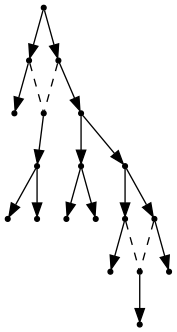
\includegraphics[width=30mm, height=45mm]{base-network.png}
  \caption{Starting Network}
  \label{fig:base-network}
  \end{center}
\end{figure}



\begin{figure}
\noindent The following diagram illustrates a situation ruled out by the \textbf{Ancestral Edge Condition} wherein we try to add an edge between two edges which are ancestral to one another:
\vspace{2mm}
  \begin{center}
  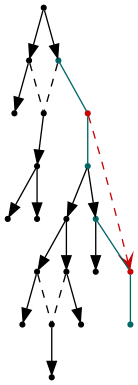
\includegraphics[width=30mm, height=55mm]{e2AncestralEdgeNetwork.png}
  \caption{Ancestral Edge Condition Violation 1}
  \label{fig:e2AncestralEdgeNetwork}
  \end{center}
\end{figure}

\FloatBarrier


\begin{figure}
\noindent Obversely we show the \textbf{Ancestral Edge Condition} wherein the target edge has a node ancestral to the source edge.
\vspace{2mm}
  \begin{center}
  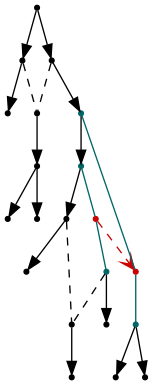
\includegraphics[width=30mm, height=55mm]{e1HasE2SrcDescendantNodeNetwork.png}
  \caption{Ancestral Edge Condition Violation 2}
  \label{fig:e1HasE2SrcDescendantNodeNetwork.png}
  \end{center}
\end{figure}

\begin{figure}
\noindent This diagram illustrates an attempt to add a network edge where the target edge is incident to a network node i.e. a situation rules out by the \textbf{Network Incident Node Condition}:
\vspace{2mm}
  \begin{center}
  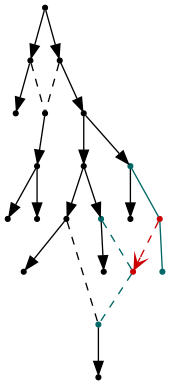
\includegraphics[width=30mm, height=45mm]{hasE2IncidentNetworkNode.png}
  \caption{Network Incident Node Condition Violation}
  \label{fig:hasE2IncidentNetworkNode}
  \end{center}
\end{figure}


\begin{figure}
\noindent Finally we illustrate the \textbf{Network Node Partner Condition}:
\vspace{2mm}
  \begin{center}
  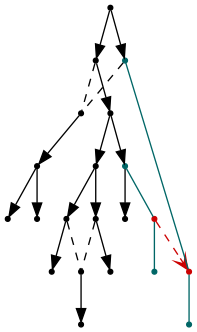
\includegraphics[width=30mm, height=45mm]{e2NetworkEdgeComplementNodeAncestralToE1.png}
  \caption{Network Node Partner Condition}
  \label{fig:e2NetworkEdgeComplementNodeAncestralToE1}
  \end{center}
\end{figure}


\begin{figure}
\subsubsection{Network Incident Node Condition}
It is worth explaining this condition further. 
Suppose we were to allow such an edge to be added as follows:

  \begin{center}
  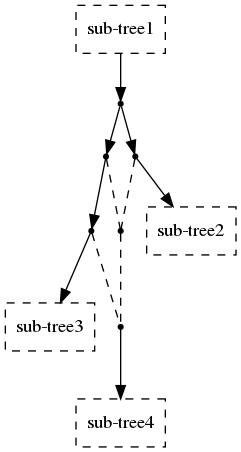
\includegraphics[width=40mm, height=65mm]{disallowed-display-network1.png}
  \caption{Invalid Phylogenetic Network Configuration}
  \label{fig:disallowed-display-network1}
  \end{center}
\end{figure}


\begin{figure}
This would then have the following display tree:
  \begin{center}
  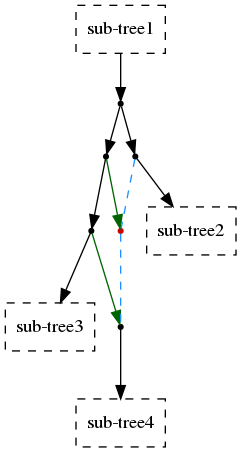
\includegraphics[width=40mm, height=65mm]{disallowed-display-tree1.png}
  \caption{Invalid Phylogenetic Tree}
  \label{fig:disallowed-display-tree1.png}
  \end{center}

Note in particular that we have \textit{added} a new leaf node in this display tree, something we wish to rule out.
\end{figure}

\newpage
\singlespacing
\bibliography{/users/ward/home/biblio/ward_new}
%\bibliography{ward_new}

%cost of root for pars = insert all characters, good first aapprox

%
%Algorithm basic template
%	\begin{algorithm}
%		\caption{Blah}
%		\label{alg:Blah}
%		\SetAlgoLined
%		\KwData{Input data $D$}
%		\KwResult{Blah}
%		\Comment{Blah Comment}
%		\Return{Bleh} 					
%	\end{algorithm}

\end{document}
